\section{实验}
\label{sec:experiments}

我们评估三个互补性问题：残差化是否降低确切条件梯度协方差，其可观测效应在在线训练过程中是否持续存在，以及由此产生的策略是否提升下游性能。我们首先明确实验协议，随后展示冻结前缀审计、数学结果与诊断分析、跨领域迁移，以及对支持集大小、回溯采样、学习率和尾部内控制的受控消融实验。

\subsection{实验设置}
\label{sec:ex-setup}

\paragraph{离线机制审计。}
我们冻结 Qwen3.5 \citep{qwen3.5} 模型，在选定的冻结数学前缀下，每个提示采样一条 64-token 轨迹，测量协方差迹和信噪比：
NSR=$\frac{\mathcal{V}(\hat{\bgrad})}{\|\bgrad_{\text{full-rKL}}\|_2^2}$ 。实验涵盖五种情景：GSM8K \citep{cobbe2021gsm8k}（32 个提示）在 0.8B/4B、4B/27B 和 9B/27B 组合中；全部 33 个 HMMT26 提示 \citep{dekoninck2026matharena}（4B/27B）；以及从 DeepMath-103K \citep{deepmath} 中采样的 64 个提示（4B/27B）。

\paragraph{在线门诊训练数学推理。}
我们从Qwen3.5-27B教师模型中蒸馏出具备思考能力的Qwen3.5-4B学生模型。从DeepMath-103K出发，我们在去重和基准污染移除后筛选出具有挑战性的竞赛问题。为确保适当的师生能力差距，我们保留教师模型在采样生成中成功两次而学生模型至少失败一次的提示。这产生了1,276个独特问题，划分为1,024个用于训练和252个用于条件性留出评估。训练运行3个轮次（192步），在第6、32、64、128和192步保存中间检查点。
\vspace{-4mm}

\paragraph{评估。}
我们的评估涵盖四个基准：DeepMath 留出集、AIME26（30 道题）\citep{aime26}、HMMT26（33 道题）\citep{dekoninck2026matharena}，以及 OlymMATH 的英文划分（200 道题）\citep{sun2025challengingboundariesreasoningolympiadlevel}。由于 AIME26 和 HMMT26 的题目数量有限，我们对每道题报告 16 次采样响应的平均值（avg@16）以缓解评估方差，而 DeepMath 留出集和 OlymMATH 使用 avg@2。除了最终性能外，我们还评估所有中间保存的检查点，以计算曲线下面积（AUC），量化学习动态和训练效率。我们在保存的检查点轨迹上计算规范化的梯形 AUC，并对每个基准的得分和 AUC 进行平均，得到汇总列。训练与评估的完整配置详见附录~\ref{app:hyperparameters}。
\vspace{-4mm}

\paragraph{实现的滚动分布。}
根据 Qwen3.5 官方配方，主要的数学推理和评估使用温度 $1.0$、top-$p=0.95$ 和 top-$k=20$。  
截断低概率 token 有助于避免导致 OPD 和教师反馈~\citep{fu2026revisiting} 不稳定的退化前缀。  
训练中使用的学生端概率通过一次全新的、未截断的前向传播重新计算。如第~\ref{subsec:evidence} 节所述，这种设置保持了明确的采样方差对比，但不满足理想化的全 rKL 无偏假设。  
因此，我们还报告了一个匹配的全支持数学消融实验（第~\ref{sec:rollout-ablation} 节）以及使用 top-$p=1.0$、top-$k=-1$ 的跨领域训练（第~\ref{sec:cross-domain} 节）。


\subsection{确切的冻结前缀协方差审计}
\label{sec:exact-audit}

\begin{table}[t]
\caption{
确切的冻结前缀协方差迹和NSR。学生Logit梯度的协方差迹通过完整动作枚举计算，并在轨迹间取平均；NSR将每个迹除以全-rKL梯度的平方$L_2$范数进行归一化。稀疏估计量($\text{vOPD}_{\text{T-Top-}k}$, HETS, ResOPD) 共享一个相同的教师预算$k=4$，其中$\text{vOPD}_{\text{T-Top-}k}$ 在此支持集上采用分离的条件-KL基准。每行最佳结果用\textbf{粗体}表示，次佳结果用\underline{下划线}表示。
}
\label{tab:mechanism}
\centering
\small
\setlength{\tabcolsep}{2.8pt}
\renewcommand{\arraystretch}{1.18}

\begin{tabular*}{\linewidth}{@{\extracolsep{\fill}}ll cccc cccc@{}}
\toprule
\multirow{2}{*}{\textbf{Dataset}}
& \multirow{2}{*}{\textbf{Models}}
& \multicolumn{4}{c}{\textbf{Covariance Trace} $\downarrow$}
& \multicolumn{4}{c}{\textbf{NSR} $\downarrow$} \\
\cmidrule(lr){3-6} \cmidrule(l){7-10}
&
& \shortstack{Sampled} & \shortstack{$\text{vOPD}_{\text{T-Top-}k}$} & \shortstack{HETS} & \shortstack{ResOPD}
& \shortstack{Sampled} & \shortstack{$\text{vOPD}_{\text{T-Top-}k}$} & \shortstack{HETS} & \shortstack{ResOPD} \\
\midrule
GSM8K    & 0.8B\,/\,4B  & 2.146 & 1.730 & \underline{1.559} & \textbf{1.018} & 5.422 & 4.370 & \underline{3.940} & \textbf{2.573} \\
GSM8K    & 9B\,/\,27B   & 0.215 & 0.192 & \underline{0.107} & \textbf{0.068} & 6.202 & 5.560 & \underline{3.101} & \textbf{1.955} \\
GSM8K    & 4B\,/\,27B   & 0.333 & 0.297 & \underline{0.183} & \textbf{0.108} & 6.058 & 5.400 & \underline{3.335} & \textbf{1.964} \\
HMMT26   & 4B\,/\,27B   & 0.208 & 0.189 & \underline{0.092} & \textbf{0.052} & 6.589 & 5.977 & \underline{2.914} & \textbf{1.630} \\
DeepMath & 4B\,/\,27B   & 0.183 & 0.169 & \underline{0.087} & \textbf{0.047} & 7.352 & 6.785 & \underline{3.500} & \textbf{1.907} \\
\bottomrule
\end{tabular*}
\end{table}

表~\ref{tab:mechanism} 报告了五个冻结前缀面板中的确切协方差迹和NSR。通过在每个学生访问的前缀处解析枚举每一个下一个token的动作，我们隔离了每个估计量的条件采样方差，而不受解码噪声或优化器反馈的影响。在表格中使用的面板级聚合下，这两个指标在每个面板中均表现出一致的排序：$\text{ResOPD} < \text{HETS} < \text{vOPD} < \text{sampled-token OPD}$（越低越好）。相对于采样token的OPD，整体协方差迹在payload匹配的Teacher-Top-$k$ vOPD中减少了$7.7\%\text{--}19.4\%$，\gzero{}中减少了$27.3\%\text{--}55.8\%$，ResOPD中减少了$52.5\%\text{--}75.0\%$。

尽管教师-顶端-$k$ vOPD 在我们的端到端实验中作为具有竞争力的基准（表~\ref{tab:math-terminal}），但其分离的标量控制无法利用结构化的头--尾分解，导致每一步都对整个动作向量进行采样。因此，与 HETS 和 ResOPD 相比，其方差减小效果仍然有限。由于 HETS 和 ResOPD 具有相同的负载预算、确切的前四名头集成以及条件目标结构，它们之间的对比能够直接隔离粗尾残差化带来的增益，而不受基准干扰。因此，我们主要关注从 HETS 到 ResOPD 的演进过程。

随着支持大小 $k$ 增加，确切的 Top-$k$ 头吸收了更多的概率质量，导致剩余尾部机会 $P\tau_p$ 缩小。相应地，ResOPD 相对于 \gzero{} 的边际协方差减小逐渐变窄。附录~\ref{app:fixed-prefix-sweep} 中的完整支持大小扫描直接测试了这种通信--方差权衡。

\subsection{端到端的数学推理}
\label{sec:math-opd}

\begin{table}[t]
\caption{
Qwen3.5-27B-to-4B OPD结果。DeepMath的保留测试集和OlymMATH使用avg@2进行评估，而AIME26和HMMT26由于题目数量较少，采用avg@16进行评估。
}
\label{tab:math-terminal}
\centering
\small
\setlength{\tabcolsep}{3.5pt}
\renewcommand{\arraystretch}{1.18}

\newcolumntype{Y}{>{\centering\arraybackslash}X}

\begin{tabularx}{\linewidth}{l YYYYY Y}
\toprule
\multirow{2}{*}[-2ex]{\textbf{Method}}
& \multicolumn{4}{c}{\textbf{Benchmark Accuracy (\%)}}
& \multicolumn{2}{c}{\textbf{Aggregate (\%)}} \\
\cmidrule(lr){2-5} \cmidrule(l){6-7}
& \shortstack{DeepMath\\{\scriptsize held-out (avg@2)}}
& \shortstack{AIME26\\{\scriptsize(avg@16)}}
& \shortstack{HMMT26\\{\scriptsize(avg@16)}}
& \shortstack{OlymMATH\\{\scriptsize(avg@2)}}
& \shortstack{Avg.\\Score}
& \shortstack{Avg.\\AUC} \\
\midrule

\rowcolor{gray!18}\multicolumn{7}{@{}l}{\textit{\textbf{$\blacktriangledown$ Original Models}}} \\
Qwen3.5-4B Student   & 48.41 & 56.25 & 35.23 & 31.50 & 42.85 & -- \\
Qwen3.5-27B Teacher  & 89.29 & 80.62 & 62.88 & 63.25 & 74.01 & -- \\

\midrule
\rowcolor{gray!18}\multicolumn{7}{@{}l}{\textit{\textbf{$\blacktriangledown$ Alternative Sparse OPD (Biased)}}} \\
Teacher Top-$k$ fKL  & 50.20 & 54.58 & 35.04 & 34.50 & 43.58 & 42.80 \\
Teacher Top-$k$ rKL  & 51.79 & 55.83 & 34.66 & 36.75 & 44.76 & 44.63 \\
TA-OPD               & 58.13 & 58.96 & \underline{39.58} & 36.00 & 48.17 & \underline{47.94} \\

\midrule
\rowcolor{gray!18}\multicolumn{7}{@{}l}{\textit{\textbf{$\blacktriangledown$ Unbiased rKL Estimators}}} \\
Sampled-token OPD    & 48.21 & 57.50 & 36.17 & 34.25 & 44.03 & 46.69 \\
vOPD$_{\text{T-Top-}k}$ & \underline{58.93} & \textbf{60.00} & 39.20 & \underline{37.25} & \underline{48.85} & 47.49 \\
\gzero{}             & 54.76 & 56.25 & 37.88 & 34.00 & 45.72 & 46.18 \\

\rowcolor{lineblue!15}
\textbf{\method{}} (\textit{ours}) & \textbf{60.91} & \underline{59.38} & \textbf{39.96} & \textbf{40.25} & \textbf{50.12} & \textbf{47.96} \\
\bottomrule
\end{tabularx}
\end{table}

表~\ref{tab:math-terminal} 报告了主要的蒸馏结果：在所有评估的OPD基准中，ResOPD实现了最强的综合性能，达到了最高的终端平均得分（50.12\%）和学习轨迹AUC（47.96\%）。这种有利的训练轨迹也延伸至外部数学竞赛。在AIME26、HMMT26和OlymMATH中，其他竞争基准在训练后期表现出明显的峰值后退化，而ResOPD则避免了严重的后期退化，并在最终检查点恢复到其最佳综合性能。中间检查点的分步评估结果在附录~\ref{app:math-learning-trajectories} 中提供并进行了分析。

\subsubsection{训练动态}
\label{sec:train_dynamics}

\begin{table}[t]
\centering
\small
\caption{\textbf{训练过程中的聚合在线诊断}（越低越好）。数值表示所有192个最优化步骤的平均值。$\Delta$ 表示相对于HETS，ResOPD的相对降低百分比。}
\label{tab:stable-dynamics}
\renewcommand{\arraystretch}{1.18}
\setlength{\tabcolsep}{6pt}
\begin{tabular}{lccccc}
\toprule
\textbf{Diagnostic Metric} & \textbf{Top-$k$ rKL} & \textbf{$\text{vOPD}_{\text{T-Top-}k}$} & \textbf{HETS} & \textbf{ResOPD (\textit{ours})} & \textbf{$\Delta$ (\%)$\downarrow$} \\
\midrule
Support-mass gap ($\times10^{-3}$)          & 11.17 & 3.53  & 5.17  & \textbf{3.50}  & $-32.3\%$ \\
$|$Tail log-mass mismatch$|$                 & 0.715 & 0.858 & 0.723 & \textbf{0.322} & $-55.5\%$ \\
Token residual $M_2$ ($\times10^{-3}$)      & --    & \textbf{10.55} & 11.73 & {10.67} & $-9.0\%$  \\
Trajectory residual $M_2$ ($\times10^{-5}$) & --    & 2.76  & 3.50  & \textbf{2.65}  & $-24.3\%$ \\
\bottomrule
\end{tabular}
\vspace{-3mm}
\end{table}

\begin{figure}[t]
\centering
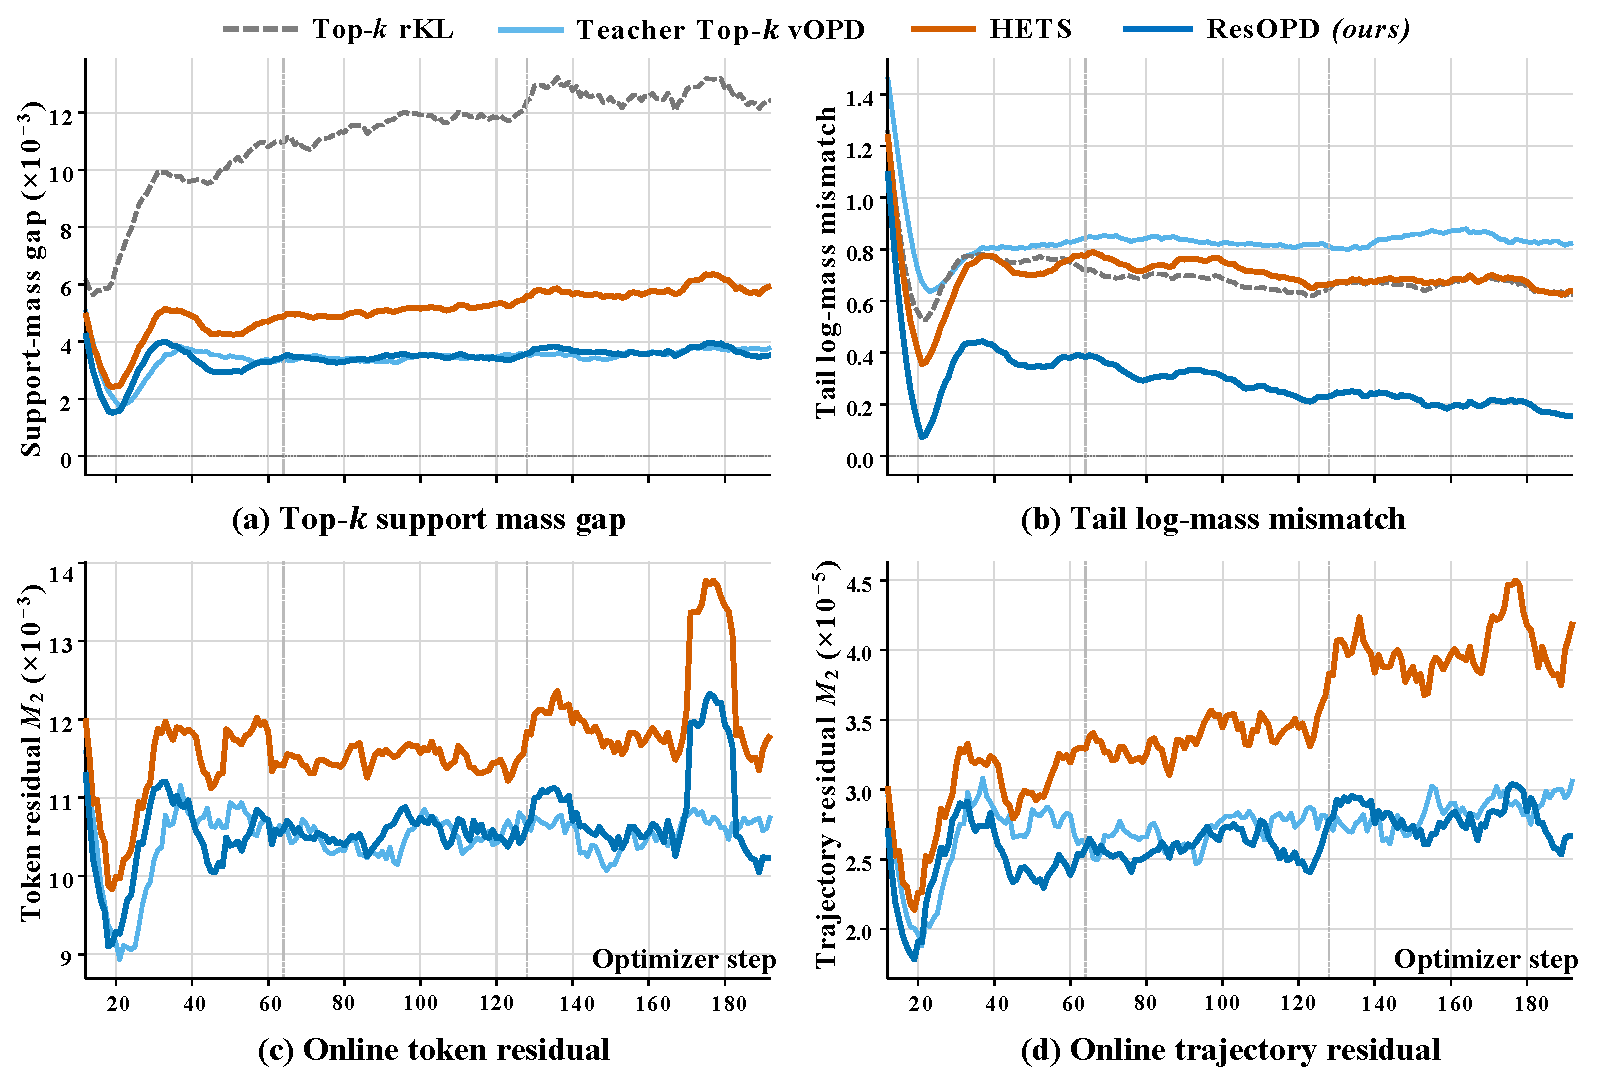
\includegraphics[width=0.85\textwidth]{figs/math_dynamics_v10.pdf}
\caption{\textbf{训练时诊断}（64步/轮次；越低越好）。
\textbf{子图(a)和(b)}展示了在vOPD、HETS、ResOPD和直接教师Top-$k$ rKL中，学生--教师不匹配在Top-$k$支撑质量和尾部对数质量上的情况。
\textbf{子图(c)和(d)}分别通过二值Top-$k$指示器与其学生预测概率之间的平方残差，在token级别和轨迹级别上比较vOPD、HETS和ResOPD。详细公式见附录~\ref{app:online-residual-moments}。}
\label{fig:training-dynamics-event-g0}
\vspace{-6mm}
\end{figure}

如表~\ref{tab:stable-dynamics} 和图~\ref{fig:training-dynamics-event-g0} 所示，与 HETS 相比，ResOPD 在平均 192 个训练步骤中持续抑制了学生-教师质量差异以及随机残差波动。在匹配的 HETS--ResOPD 运行中，ResOPD 将支持质量差距减少了 $32.3\%$ ，并将尾部对数质量不匹配减少了 $55.5\%$ 。尽管 Teacher-Top-$k$ vOPD 展现了相当的支持事件 $M_2$ ，但其在自生成轨迹上的标量残差忽略了中心化对数比和得分几何结构，且在共享冻结前缀上的确切梯度协方差比较（表~\ref{tab:mechanism}）确认了 ResOPD 的结构优势。

这为ResOPD的最优化行为提供了机制性解释。在HETS下，完整的微调尾部梯度修正集中在稀有尾部命中事件上。尽管头部覆盖度约为$98.4\%$，一个$30\text{K}$-token推理迹中仍包含460–470次此类修正，每轮优化器步骤累积达数千次。通过减去可用载荷的尾部桶分量$\bmean_B$，ResOPD在保留同策略条件下第Sec.~\ref{subsec:evidence}中全-rKL期望的同时，重新分配了事件间的可预测成分。下游准确率仍然存在更多噪声，因为它依赖于离散答案的正确性，但仅完成情况的教师NLL审计显示，ResOPD生成的学生轨迹具有更一致更高的教师似然。结合匹配的终点与曲线-AUC结果，这些诊断将估计量层面的协方差减小与更平滑的最优化路径及改进的下游性能联系起来。

\vspace{-4mm}
\subsubsection{行为忠实性}
\label{sec:math-eval-diagnostics}

除了特定任务的准确率指标（例如在下游数学基准上的avg@2和avg@16），监控学生模型在教师模型下的负对数似然值，可以提供一种内在的、与任务无关的蒸馏保真度读数。具体而言，教师模型的较低负对数似然值表明学生样本在教师模型下的似然值更高。

图~\ref{fig:teacher-nll} 跟踪了该度量在匹配的数学运行过程中的变化。如面板~A所示，尽管两种估计量初始值均约为 $0.46$ \,nats/token，但ResOPD在第6步时下降更为迅速，并持续保持单调下降趋势，至第192步时降至 $0.36$ \,nats/token。相比之下，HETS在约 $0.385$ \,nats/token 处趋于平稳，并在后期表现出轻微漂移。在面板~B中，二者之差 $\Delta\text{Teacher-NLL (ResOPD} - \text{HETS)}$ 在所有优化器步骤中始终保持负值，并扩大至超过 $-0.027$ \,nats/token。这表明ResOPD始终比HETS更有效地保持与教师模型的行为一致性，提供了更高教师相似性的证据，与准确率形成互补。


\subsection{跨领域迁移至科学与编程}
\label{sec:cross-domain}

\begin{figure}[htbp]
\centering
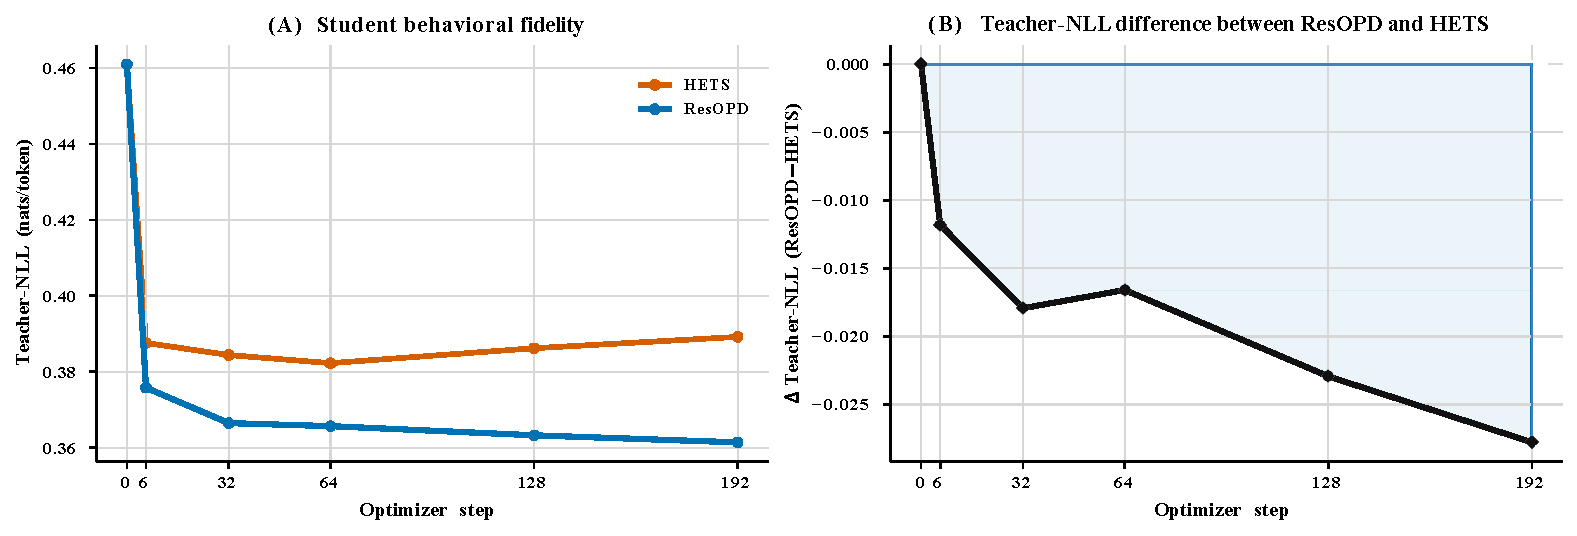
\includegraphics[width=0.9\textwidth]{figs/teacher_nll_fidelity_v3.pdf}
\vspace{-2mm}
\caption{\textbf{Math OPD 设置下训练过程中教师的负对数似然（NLL）}。  
评估在四个核心基准族上进行，权重与主套件相同：AIME26、HMMT26、DeepMath 留出集和 OlymMATH。数值越低，表示对教师分布的保真度越高。}
\label{fig:teacher-nll}
\end{figure}

\begin{table}[h]
\caption{
Qwen3-30B-A3B-Instruct到Qwen3-4B的蒸馏结果。评估使用GPQA-D的avg@10，以及SuperGPQA、LCB-v5和LCB-v6的avg@3。AUC综合了固定训练轨迹（Base/10/25/50/100）上的性能表现。
}
\label{tab:qwen3-transfer}
\centering
\small
\setlength{\tabcolsep}{3.5pt}
\renewcommand{\arraystretch}{1.18}

\newcolumntype{Y}{>{\centering\arraybackslash}X}

\begin{tabularx}{\linewidth}{l YYYY YY}
\toprule
\multirow{2}{*}[-2ex]{\textbf{Method}}
& \multicolumn{2}{c}{\textbf{Science Benchmarks (\%)}}
& \multicolumn{2}{c}{\textbf{Code Benchmarks (\%)}}
& \multicolumn{2}{c}{\textbf{Aggregate (\%)}} \\
\cmidrule(lr){2-3} \cmidrule(lr){4-5} \cmidrule(l){6-7}
& \shortstack{GPQA-D\\{\scriptsize(avg@10)}}
& \shortstack{SuperGPQA\\{\scriptsize(avg@3)}}
& \shortstack{LCB-v5\\{\scriptsize(avg@3)}}
& \shortstack{LCB-v6\\{\scriptsize(avg@3)}}
& \shortstack{Avg.\\Score}
& \shortstack{Avg.\\AUC} \\
\midrule

\rowcolor{gray!18}\multicolumn{7}{@{}l}{\textit{\textbf{$\blacktriangledown$ Original Models}}} \\
Student             & 45.25          & 32.46          & 21.76          & 24.38          & 30.96          & -- \\
Teacher             & 56.06          & 48.87          & 45.51          & 41.71          & 48.04          & -- \\

\midrule
\rowcolor{gray!18}\multicolumn{7}{@{}l}{\textit{\textbf{$\blacktriangledown$ Unbiased rKL Estimators}}} \\
Sampled-token OPD   & \textbf{50.30} & \underline{36.87} & 43.31          & 39.43          & 42.48          & 41.21 \\
HETS                & \underline{48.89} & 36.10          & \underline{46.31} & \textbf{43.24} & \underline{43.63} & \underline{42.13} \\

\rowcolor{lineblue!15}
\textbf{ResOPD} (\textit{ours}) & 47.12          & \textbf{37.54} & \textbf{48.90} & \underline{43.05} & \textbf{44.15} & \textbf{42.65} \\
\bottomrule
\end{tabularx}
\end{table}

为了进一步评估 ResOPD 的泛化能力与跨领域有效性，我们遵循 \citet{heo2026policy} 并将研究范围扩展至科学和编程任务。我们的实验协议在很大程度上模仿了 \citet{heo2026policy}：从一个 Qwen3-30B-A3B-Instruct \citep{yang2025qwen3} 教师模型中蒸馏出一个 Qwen3-4B 学生模型，训练数据为由 OpenMathReasoning \citep{moshkov2025aimo}、OpenScienceReasoning-2 \citep{nvidia2025opensciencereasoning2} 和 OpenCodeReasoning \citep{ahmad2025opencodereasoning} 构成的 30k 样本混合数据集。运行过程中采用全支持的祖先回溯（ancestral rollouts），温度 $1.0$，top-$p=1.0$ 和 top-$k=-1$，不启用思考模式。在评估方面，我们在代码领域上基于 LiveCodeBench \citep[LCB;][]{jain2025livecodebench} v5（167 个问题）和 v6（175 个问题）进行基准测试。在科学领域，我们在 GPQA-Diamond \citep[GPQA-D, 198 problems;][]{rein2023gpqa} 和 SuperGPQA \citep{du2026supergpqa} 上进行评估，采用 \citet{heo2026policy} 中使用的 650 个问题的确切子集。

表~\ref{tab:qwen3-transfer} 报告了评估结果。总体而言，ResOPD 在各项指标上均表现最强，分别在终端平均得分（$44.15\%$）和轨迹 AUC（$42.65\%$）上领先。尽管 ResOPD 和 HETS 在代码任务上看似超越了教师模型（例如，ResOPD 的 $48.90\%$ 与 $45.51\%$ 在 LCB-v5 上的表现），但配对的自助法 95\% 置信区间跨越零点（例如，ResOPD$-$ 与教师模型在 LCB-v6 上的差异范围为 $[-2.48, +5.33]$），表明其性能与教师模型相当，并未体现出统计上显著的超教师泛化能力。

在不同训练规模下，ResOPD 均保持一致的优化优势（例如，将轨迹残差 $M_2$ 减少 $9.5\%$ --$12.6\%$ ，梯度范数减少 $14.6\%$ --$23.7\%$ ），并在代码任务上对 HETS 显现出方向性 AUC 提升（$+0.48$ 与 $+0.73$ 点），尽管采样 token 的 OPD 在科学任务上表现最佳（详细训练检查点曲线见附录~\ref{app:cross-qwen3}）。
\vspace{-2mm}

\subsection{在线支持大小消融}
\label{sec:online-support}

\begin{table}[t]
\caption{不同 Top-$k$ 支持大小下的性能（匹配单轮次预算）。评估设置遵循表~\ref{tab:math-terminal}（AIME26/HMMT26 的 avg@16，OlymMATH 的 avg@2）。$\Delta$ 表示 ResOPD 相对于 HETS 的平均提升。}
\label{tab:topk-breakdown}
\centering
\small
\renewcommand{\arraystretch}{1.1}

\begin{tabular*}{0.80\textwidth}{@{\extracolsep{\fill}}cc cccc c@{}}
\toprule
\textbf{$k$} & \textbf{Method} & \textbf{AIME26} & \textbf{HMMT26} & \textbf{OlymMATH} & \textbf{Average} & \textbf{$\Delta$} \\
\midrule
\multirow{2}{*}{1}
& HETS & \textbf{60.62} & 37.69          & 34.75          & 44.35          & \multirow{2}{*}{$+0.11$} \\
& ResOPD  & 56.88          & \textbf{39.02} & \textbf{37.50} & \textbf{44.47} & \\
\addlinespace[3pt]
\multirow{2}{*}{4}
& HETS & 59.17          & 36.93          & 34.50          & 43.53          & \multirow{2}{*}{$+1.01$} \\
& ResOPD  & \textbf{60.00} & \textbf{37.88} & \textbf{35.75} & \textbf{44.54} & \\
\addlinespace[3pt]
\multirow{2}{*}{16}
& HETS & 57.92          & \textbf{39.39} & 35.75          & 44.35          & \multirow{2}{*}{$+0.70$} \\
& ResOPD  & \textbf{59.38} & 39.02          & \textbf{36.75} & \textbf{45.05} & \\
\addlinespace[3pt]
\multirow{2}{*}{32}
& HETS & 59.79          & \textbf{39.02} & 36.75          & 45.19          & \multirow{2}{*}{$+1.56$} \\
& ResOPD  & \textbf{61.67} & 38.07          & \textbf{40.50} & \textbf{46.75} & \\
\bottomrule
\end{tabular*}
\end{table}

\begin{figure}[t]
\centering
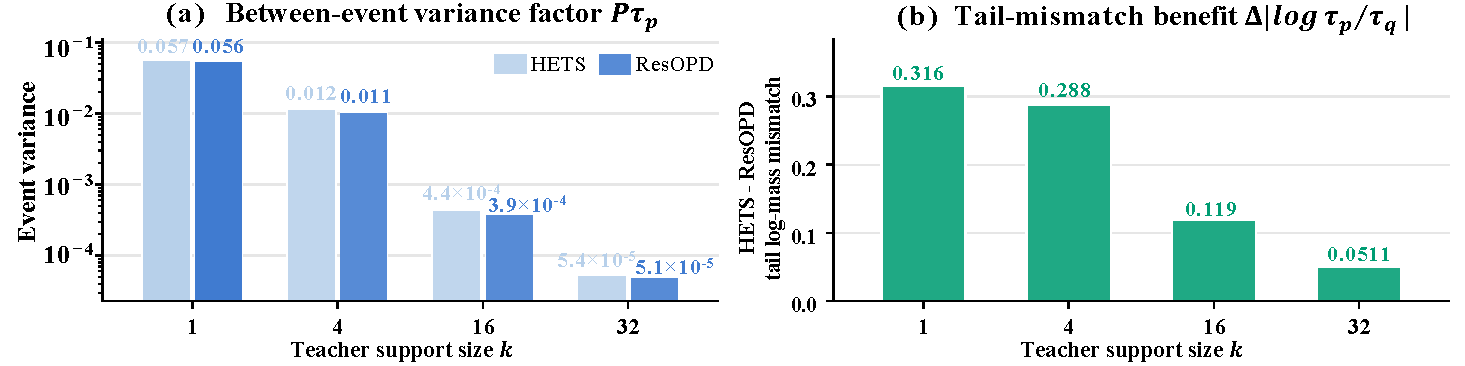
\includegraphics[width=0.9\textwidth]{figs/topk_ablation_v10.pdf}
\caption{在线诊断指标在教师模型 Top-$k$ 支持大小上的表现。
\textbf{(a)} HETS 和 ResOPD 的事件间方差因子 $P\tau_p$，表征头部与尾部划分的缩放系数。
\textbf{(b)} 尾部对数质量不匹配的减少量 ($\text{HETS} - \text{ResOPD}$，通过 $\Delta|\log(\tau_p / \tau_q)|$ 测量)。}
\label{fig:topk-ablation}
\vspace{-4mm}
\end{figure}

附录~\ref{app:fixed-prefix-sweep} 在固定前缀的情况下，研究了支持集大小 $k$ 的影响，报告了确切的协方差迹和NSR。相比之下，此处我们提供了对OPD的端到端在线消融分析。具体而言，表~\ref{tab:topk-breakdown} 和图~\ref{fig:topk-ablation} 展示了在不同教师支持集大小 $k \in \{1, 4, 16, 32\}$ 下的结果。  
如表~\ref{tab:topk-breakdown} 所示，ResOPD 在所有测试的支持集大小下，平均下游准确率均优于HETS，提升幅度从 $+0.11$ 个百分点（在 $k=1$ 处）到 $+1.56$ 个百分点（在 $k=32$ 处）不等。  
然而，尽管下游任务得分始终青睐ResOPD，但ResOPD所提供的内在方差减小优势预计会随着 $k$ 增大而减弱，因为更大的教师支持集自然能捕捉更多的概率质量，从而使得尾部修正的发生频率降低。

图~\ref{fig:topk-ablation} 验证了该机制在表~\ref{tab:topk-breakdown} 所示运行结果中的有效性。在图~\ref{fig:topk-ablation}(a) 中，HETS 和 ResOPD 的方差因子 $P\tau_p$ 几乎相同，均从 $k=1$ 降至 $32$ 以下三个数量级。这直接反映了理论上的 ResOPD--HETS 方差对比与尾部-均值近似质量之间的比例关系。同时，图~\ref{fig:topk-ablation}(b) 显示，ResOPD 在所有支持范围内始终降低了尾部对数质量不匹配度，尤其在紧支持区域的差异最为显著。

\subsection{Rollout采样：默认过滤器与完整支持}
\label{sec:rollout-ablation}
尽管在我们的确切枚举审计（第~\ref{sec:exact-audit} 节）和跨领域迁移实验（第~\ref{sec:cross-domain} 节）中严格遵守了理想化的原始采样条件 $A\sim p_\theta$，我们仍为完整性验证了主要数学结果不依赖于轨迹截断。具体而言，在保持所有其他训练超参数不变的情况下，我们在全支持采样 ($\text{top-}p=1.0$ , $\text{top-}k=-1$ ) 下评估了首个训练轮次。

如表~\ref{tab:full-support-first-epoch} 所示，移除轨迹过滤器后，所有三种评估方法的 AUC 均下降。然而，ResOPD 在基准准确率和轨迹 AUC 两个方面始终优于 HETS 和朴素基准。此外，我们观察到移除轨迹过滤器会导致更长的推理轨迹，并在训练过程中更高频率地触及响应 token 限制。


\subsection{学习率敏感性}
\label{sec:lr-sensitivity}

\begin{table}[t]
\centering
\small
\caption{\textbf{默认滚动与全支持滚动下的首轮次数学性能。}
基准得分和平均值表示第64步的准确率（\%）；$\text{AUC}$ （\%）衡量步骤 $\{0, 6, 32, 64\}$ 内规范化学习曲线面积；  
\textit{默认}：前-$p=0.95$ ，前-$k=20$ ；\textit{全支持}：前-$p=1.0$ ，前-$k=-1$ 。}
\vspace{-2mm}
\label{tab:full-support-first-epoch}
\setlength{\tabcolsep}{5pt}
\renewcommand{\arraystretch}{1.15}
\begin{tabular}{llcccccc}
\toprule
\textbf{Rollout} & \textbf{Method} & \textbf{DeepMath} & \textbf{AIME26} & \textbf{HMMT26} & \textbf{OlymMATH} & \textbf{Avg.} & \textbf{AUC} \\
\midrule
\multirow{3}{*}{Default}
& Naive Top-$k$ rKL & 53.17 & 56.04 & 35.42 & 35.00 & 44.91 & 45.45 \\
& HETS              & 53.17 & 59.17 & 36.93 & 34.50 & 45.94 & 46.12 \\
& ResOPD            & \textbf{54.76} & \textbf{60.00} & \textbf{37.88} & \textbf{35.75} & \textbf{47.10} & \textbf{47.57} \\
\midrule
\multirow{3}{*}{Full}
& Naive Top-$k$ rKL & 45.44 & 55.42 & 35.80 & 34.25 & 42.72 & 44.96 \\
& HETS              & 49.80 & 57.50 & \textbf{37.88} & 35.50 & 45.17 & 45.68 \\
& ResOPD            & \textbf{57.14} & \textbf{60.42} & \textbf{37.88} & \textbf{36.00} & \textbf{47.86} & \textbf{46.79} \\
\bottomrule
\end{tabular}
\end{table}

\paragraph{实验设置与评估协议。}
为了评估在激进步长下的最优化鲁棒性，我们进行了一次受控的学习率扫描（$k=4$），其设置与主数学实验一致，不同之处在于训练被压缩至1~轮次（64次优化器步骤）。所有实验均采用批量大小为16、32K响应预算，并与主实验保持相同的采样配置。在步骤0、6、32和64处的检查点均按照宏-4协议进行评估（对AIME26和HMMT26平均采样16个响应，对DeepMath保留集和OlymMATH采样2个响应）。
\vspace{-4mm}

\begin{table}[t]
\centering
\small
\caption{\textbf{HETS 与 ResOPD 的学习率敏感性。} $\Delta$ 表示 ResOPD 相对于 HETS 的提升。}
\vspace{-2mm}
\label{tab:lr-sensitivity}
\renewcommand{\arraystretch}{1.18}
\setlength{\tabcolsep}{7pt}
\begin{tabular}{@{}l cc c cc c@{}}
\toprule
\multirow{2}{*}{\textbf{Learning Rate}}
& \multicolumn{3}{c}{\textbf{Final Score (\%)}}
& \multicolumn{3}{c}{\textbf{Trajectory AUC (\%)}} \\
\cmidrule(lr){2-4} \cmidrule(l){5-7}
& HETS & ResOPD & $\Delta$
& HETS & ResOPD & $\Delta$ \\
\midrule
$1\times10^{-6}$ & 45.94 & \textbf{47.10} & $+1.16$ & 46.12 & \textbf{47.57} & $+1.45$ \\
$2\times10^{-6}$ & 45.94 & \textbf{46.61} & $+0.67$ & 45.69 & \textbf{46.17} & $+0.48$ \\
$5\times10^{-6}$ & 42.54 & \textbf{46.35} & \textbf{+3.81} & 43.88 & \textbf{47.77} & \textbf{+3.89} \\
\bottomrule
\end{tabular}
\vspace{-4mm}
\end{table}

\paragraph{不同学习率下的性能鲁棒性。}
如表~\ref{tab:lr-sensitivity} 所示，ResOPD 在较高的学习率下表现出显著更强的鲁棒性。当学习率缩放到 $5\times10^{-6}$ 时，HETS 出现严重退化，其最终得分从 $45.94\%$ 降至 $42.54\%$  ($-3.40\%$ )，轨迹 AUC 下降了 $2.24\%$ 。相比之下，ResOPD 保持了稳定的性能（最终得分为 $46.35\%$ ，AUC 为 $47.77\%$ ），其在最终得分上对 HETS 的领先优势扩大至 $+3.81\%$ ，在 AUC 上则扩大至 $+3.89\%$ 。

在该激进学习率下的子基准分解分析显示，ResOPD 在第 64 步的所有四个组成基准上均持续保持正向优势：在 AIME26 上为 $+3.96\%$ ，在 HMMT26 上为 $+2.08\%$ ，在 DeepMath 留出集上为 $+6.94\%$ ，在 OlymMATH 上为 $+2.25\%$ 。我们在附录~\ref{app:lr-sensitivity} 中提供了不同学习率下的详细训练动态。  
\vspace{-4mm}

\paragraph{稳定性边界与失稳模式。}
当学习率进一步缩放至 $1\times10^{-5}$ 时，两种方法均迅速发散，触发严重的梯度裁剪（HETS 为 $4/6$ 步，ResOPD 为 $5/6$ 步），并在六步优化器迭代内出现严重的响应长度坍塌。尽管 ResOPD 在我们默认的训练方案下并未改变最终的发散边界 ($1\times10^{-5}$)，但其粗粒度残差化结构在中等激进的训练环境下提供了显著更宽的稳定性裕度。超出此阈值后，可能需要将更高的学习率与互补的稳定化技术（如更大的批量大小或更紧的裁剪阈值）协同使用，这留待未来工作研究。
\vspace{-4mm}

\subsection{比较双控制终点}
\label{sec:control-comparison}

第\ref{sec:unified} 节中的分析指出，通过 $\gamma$ 可以显著降低尾部内部方差。我们使用 SC-TA ($\gamma=1$ ) 和 ResOPD ($\gamma=0$ ) 对该预测进行了评估，同时保持可观测的粗粒度控制 $\bm B=\bmean_B$ 不变。

\subsubsection{跨分布固定前缀审计}
尽管双控制框架表明，SC-TA ($\gamma=1$ ) 可以缓解 ResOPD ($\gamma=0$ ) 无法处理的尾部波动，但公式~(\ref{eq:event-improvement}) 暗示这种排序依赖于分布，并非普遍成立。为评估跨领域的稳定性，我们在三个自然提示分布（DeepMath \citep{deepmath}、MegaScience \citep{fan2025megascience} 和 SynLogic \citep{liu2026synlogic}）上固定 Qwen3.5-4B/27B 对（前4名支持，64-token 视野），对128条轨迹（8,192个前缀）进行评估，使用20,000次自举重采样。我们追踪规范化的迹方差减小：
\begin{equation}
  \Delta \coloneqq \frac{\mathcal{V}_{\mathrm{SC}} - \mathcal{V}_{\mathrm{ResOPD}}}{\mathcal{V}_{\mathrm{sampled}}},
\end{equation}
负值有利于SC-TA。

如表~\ref{tab:scta-cross-distribution} 所示，总体迹方差在所有三个评估领域中均一致地支持 SC-TA 胜过 ResOPD ($\Delta \in [-0.207, -0.126]$)。同时，前缀级别的交叉现象依然显著（在 SynLogic 中多达 $18.0\%$ 的前缀更倾向于 ResOPD）。这一实证结果验证了我们双控制公式的合理预测：尽管设定 $\gamma=1$ 可能在期望上带来更低的方差，但局部方差排序仍严格依赖于前缀，而非全局统一。

原则上，可以从前训练分布中预先选择一组提示，以经验方式校准最优系数 $\gamma^\star$，从而在最优化过程中可能实现额外的方差减小（尽管 $\gamma^\star$ 会随着模型权重自然演化）。然而，在实践中，我们的实验表明，与固定启发式方法 $\gamma=1$ 相比，这种校准带来的增量收益微乎其微。因此，为保持简洁，我们省略进一步讨论。

\begin{table}[t]
\caption{\textbf{SC-TA 与 ResOPD 在自然提示分布下的协方差迹排序对比。}}
\vspace{-2mm}
\label{tab:scta-cross-distribution}
\centering
\small
\setlength{\tabcolsep}{6.0pt}
\begin{tabular}{@{}lccc@{}}
\toprule
Dataset & $\mathcal{V}_{\mathrm{SC}} / \mathcal{V}_{\mathrm{ResOPD}}$ & $\Delta$ & ResOPD-Lower Prefixes \\
\midrule
DeepMath    & 0.512 & $-0.126$ & \phantom{0}6.8\% \\
MegaScience & 0.532 & $-0.207$ & 11.3\% \\
SynLogic    & 0.558 & $-0.161$ & 18.0\% \\
\bottomrule
\end{tabular}
\vspace{-2mm}
\end{table}

\begin{table}[t]
\caption{\textbf{训练更新过程中的匹配评估曲线（\%）。}
在 Qwen3.5-27B-to-4B 蒸馏上评估，涵盖 AIME26/HMMT26（平均@16）和保留的 DeepMath/OlymMATH（平均@2）。}
\vspace{-2mm}
\label{tab:scta-curve}
\centering
\small
\setlength{\tabcolsep}{5.5pt}
\begin{tabular}{@{}lcccccc@{}}
\toprule
Method & Base (Step 0) & Step 6 & Step 32 & Step 64 & Step 128 & Step 192 \\
\midrule
HETS  & 42.85 & \textbf{48.86} & 45.04 & 45.94 & 46.60 & 45.72 \\
ResOPD   & 42.85 & 48.23 & \textbf{47.95} & 47.10 & 47.71 & \textbf{50.12} \\
SC-TA & 42.85 & 47.66 & 46.69 & \textbf{47.26} & \textbf{48.27} & 46.33 \\
\bottomrule
\end{tabular}
\vspace{-4mm}
\end{table}

\subsubsection{下游评估对比}
虽然SC-TA将固定前缀残差协方差迹减半，但这一优势并不一定转化为下游准确率的提升。如表~\ref{tab:scta-curve}所示，SC-TA并未在下游任务中表现出对ResOPD的一致优势：在多个中间检查点上表现略强，而ResOPD在最终得分上更高，轨迹级AUC保持相近。

This decoupling between gradient covariance trace and downstream performance is informative rather than contradictory. While lower estimator variance validates the two-control residualization mechanism locally, downstream benchmark accuracy reflects the global trajectory of policy updates.
Consequently, while SC-TA exhibits lower overall variance across the evaluated audit sets, ResOPD retains strong aggregate performance in this evaluated setting without explicitly subtracting the additional within-tail score fluctuation.
\vspace{-4mm}
